\documentclass[tikz,border=5pt]{standalone}
\usepackage{tikz}
\usetikzlibrary{shapes.geometric, arrows.meta, positioning, calc}
\begin{document}
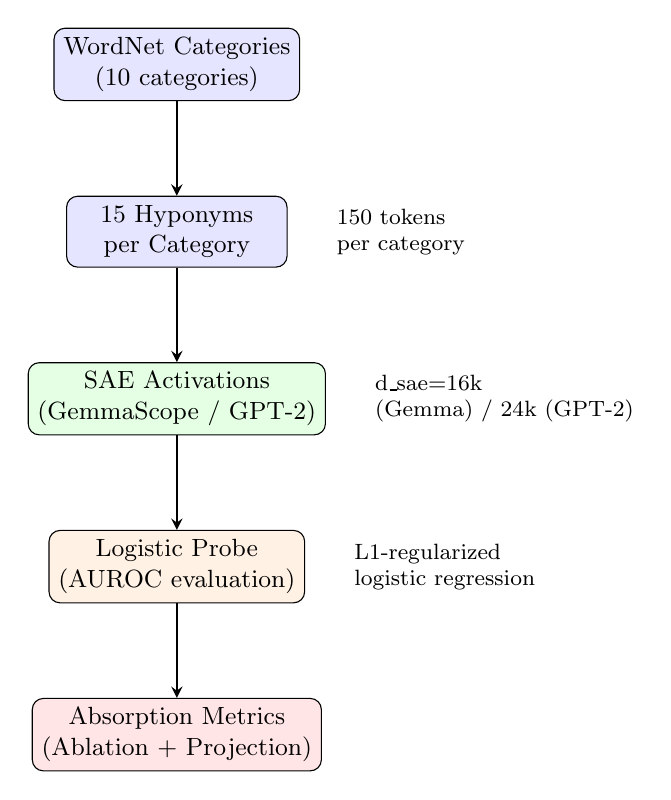
\begin{tikzpicture}[
    node distance=1.2cm,
    box/.style={rectangle, draw, rounded corners, minimum width=2.8cm, minimum height=0.9cm, align=center, font=\small},
    arrow/.style={->, >=stealth, thick},
    label/.style={font=\footnotesize\bfseries}
]
% Input
\node[box, fill=blue!10] (input) {WordNet Categories\\(10 categories)};
% Hyponyms
\node[box, fill=blue!10, below=of input] (hyponyms) {15 Hyponyms\\per Category};
% SAE
\node[box, fill=green!10, below=of hyponyms] (sae) {SAE Activations\\(GemmaScope / GPT-2)};
% Probe
\node[box, fill=orange!10, below=of sae] (probe) {Logistic Probe\\(AUROC evaluation)};
% Metrics
\node[box, fill=red!10, below=of probe] (metrics) {Absorption Metrics\\(Ablation + Projection)};
% Arrows
\draw[arrow] (input) -- (hyponyms);
\draw[arrow] (hyponyms) -- (sae);
\draw[arrow] (sae) -- (probe);
\draw[arrow] (probe) -- (metrics);
% Side labels
\node[right=0.5cm of hyponyms, font=\footnotesize, align=left] {150 tokens\\per category};
\node[right=0.5cm of sae, font=\footnotesize, align=left] {d\_sae=16k\\(Gemma) / 24k (GPT-2)};
\node[right=0.5cm of probe, font=\footnotesize, align=left] {L1-regularized\\logistic regression};
\end{tikzpicture}
\end{document}
